\documentclass[tikz,border=2pt]{standalone}
\usepackage[T1]{fontenc}
\usepackage{mathptmx}
\renewcommand{\ttdefault}{pcr}
\usepackage{tikz}
\usepackage{siunitx}
\usepackage{amssymb}
\sisetup{group-separator={,},group-minimum-digits=4}
\usetikzlibrary{positioning,arrows.meta,calc,fit,backgrounds,shapes.misc}
% palette shared with make_figs.py
\definecolor{ink}{HTML}{0B0B0B}
\definecolor{ink2}{HTML}{52514E}
\definecolor{muted}{HTML}{8A8984}
\definecolor{rule}{HTML}{E6E5E1}
\definecolor{paper}{HTML}{F7F6F3}
\definecolor{good}{HTML}{1BAF7A}
\definecolor{kh}{HTML}{E34948}
\definecolor{ball}{HTML}{EDA100}
\definecolor{lof}{HTML}{2A78D6}
\definecolor{agent}{HTML}{3D3A6B}
\definecolor{agentbg}{HTML}{EEEDF6}
\definecolor{serverbg}{HTML}{EAF3EE}
\tikzset{
  >={Stealth[length=2.2mm,width=1.6mm]},
  box/.style={draw=ink2, line width=0.5pt, rounded corners=2pt, fill=white, align=center, inner sep=3pt, font=\footnotesize},
  chip/.style={draw=ink2, line width=0.4pt, rounded corners=1.5pt, fill=white, font=\scriptsize\ttfamily, inner xsep=3pt, inner ysep=2pt, minimum height=4.2mm},
  region/.style={draw=muted, line width=0.5pt, dashed, rounded corners=4pt, inner sep=6pt},
  lab/.style={font=\scriptsize, text=ink2, align=center},
  flow/.style={->, line width=0.6pt, draw=ink2},
  ret/.style={->, line width=0.6pt, draw=ink2, densely dashed},
  bubble/.style={draw=ink2, line width=0.5pt, rounded corners=6pt, fill=paper, align=left, inner sep=4pt, font=\footnotesize},
  num/.style={circle, fill=ink, text=white, font=\tiny\bfseries, inner sep=0.8pt, minimum size=3.4mm},
}

\begin{document}
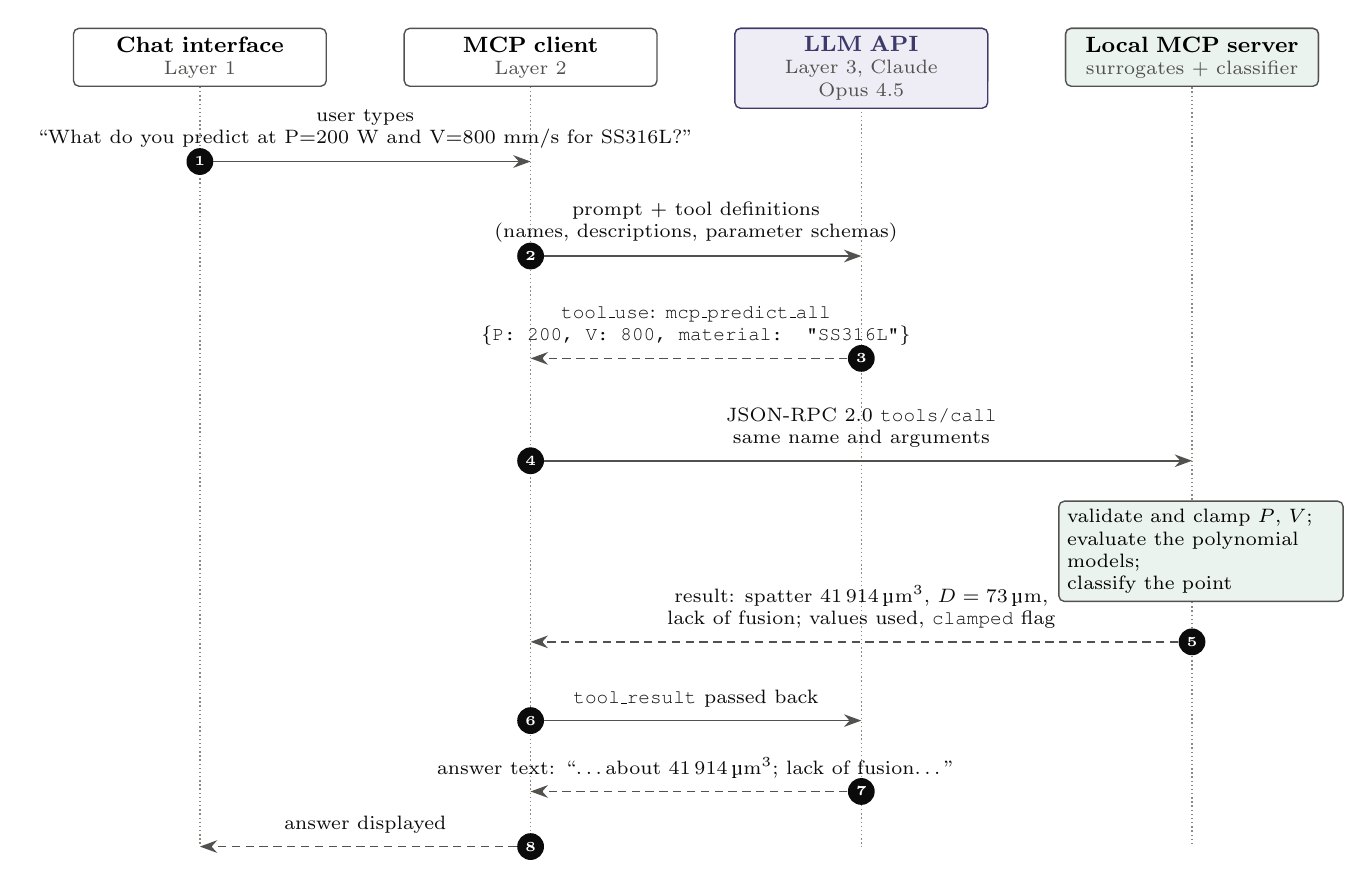
\begin{tikzpicture}
\def\top{0}\def\bot{-104mm}
% lanes: x positions
\coordinate (L1) at (0,0); \coordinate (L2) at (42mm,0); \coordinate (L3) at (84mm,0); \coordinate (L4) at (126mm,0);
\foreach \x/\n/\t/\s in {L1/h1/Chat interface/Layer 1, L2/h2/MCP client/Layer 2, L3/h3/LLM API/Layer 3, L4/h4/Local MCP server/user's machine}{
  \node[box, text width=30mm, font=\scriptsize, anchor=north] (\n) at (\x) {\textbf{\footnotesize \t}\\{\color{ink2}\s}};
  \draw[muted, line width=0.5pt, densely dotted] (\n.south) -- ($(\x)+(0,\bot)$);
}
\node[box, text width=30mm, font=\scriptsize, anchor=north, draw=agent, fill=agentbg] at (L3) {\textbf{\footnotesize\textcolor{agent}{LLM API}}\\{\color{ink2}Layer 3, Claude Opus 4.5}};
\node[box, text width=30mm, font=\scriptsize, anchor=north, fill=serverbg] at (L4) {\textbf{\footnotesize Local MCP server}\\{\color{ink2}surrogates + classifier}};

% helper: message arrow at depth y between lanes a,b with step number and label
\newcommand{\msg}[6]{% #1 y, #2 from lane, #3 to lane, #4 step, #5 label, #6 style
  \draw[#6] ($(#2)+(0,#1)$) -- ($(#3)+(0,#1)$)
    node[pos=0.5, above=0.4mm, lab, font=\scriptsize, text=ink, align=center] {#5};
  \node[num] at ($(#2)+(0,#1)$) {#4};
}
\msg{-17mm}{L1}{L2}{1}{user types\\``What do you predict at P=200 W and V=800 mm/s for SS316L?''}{flow}
\msg{-29mm}{L2}{L3}{2}{prompt + tool definitions\\(names, descriptions, parameter schemas)}{flow}
\msg{-42mm}{L3}{L2}{3}{\texttt{tool\_use}: \texttt{mcp\_predict\_all}\\\texttt{\{P: 200, V: 800, material: "SS316L"\}}}{ret}
\msg{-55mm}{L2}{L4}{4}{JSON-RPC 2.0 \texttt{tools/call}\\same name and arguments}{flow}
% server processing note
\node[box, font=\scriptsize, text width=34mm, align=left, anchor=west, fill=serverbg] (proc) at ($(L4)+(-17mm,-66.5mm)$) {validate and clamp $P$, $V$;\\evaluate the polynomial models;\\classify the point};
\msg{-78mm}{L4}{L2}{5}{result: spatter \num{41914}\,\textmu m$^3$, $D = 73$\,\textmu m,\\lack of fusion; values used, \texttt{clamped} flag}{ret}
\msg{-88mm}{L2}{L3}{6}{\texttt{tool\_result} passed back}{flow}
\msg{-97mm}{L3}{L2}{7}{answer text: ``\ldots about \num{41914}\,\textmu m$^3$; lack of fusion\ldots''}{ret}
\msg{-104mm}{L2}{L1}{8}{answer displayed}{ret}
\end{tikzpicture}
\end{document}
